\documentclass[uplatex]{jsarticle}

\usepackage{amssymb}
\usepackage{amsmath}
\usepackage{mathrsfs}
\usepackage{amsfonts}
\usepackage{mathtools}

\usepackage{xcolor}
\usepackage[dvipdfmx]{graphicx}



\usepackage{ulem}

\usepackage{braket}

%%%%%ハイパーリンク
%\usepackage[colorlinks=true,urlcolor=blue!70!black,citecolor=blue!60!black,linkcolor=blue!60!black]{hyperref}
%\usepackage{aliascnt} %for creating different biblatex references for different theoremstyles
\usepackage[setpagesize=false,dvipdfmx]{hyperref}
\usepackage{aliascnt}
\hypersetup{
    colorlinks=true,
    citecolor=blue,
    linkcolor=blue,
    urlcolor=blue,
}

\renewcommand{\eqref}[1]{\textcolor{blue}{(\ref{#1})}}

%%%%%%ハイパーリンク


%%%%%図式
%\usepackage{tikz}%%%図
\usepackage{amscd}%%%簡単な図式

\usepackage{tikz}
\usepackage{tikz-cd} %commutative diagrams in TikZ
\usetikzlibrary{calc}
\usetikzlibrary{matrix,arrows}
\usetikzlibrary{decorations.markings}

%%%%%図式



%%%%%%%%%%%%定理環境%%%%%%%%%%%%
%%%%%%%%%%%%定理環境%%%%%%%%%%%%
%%%%%%%%%%%%定理環境%%%%%%%%%%%%

\usepackage{amsthm}

%%%%%%%%%%%%Plain型%%%%%%%%%%%%


\newcommand{\myTheoremEnvironments}[1]{#1}

\myTheoremEnvironments{

%%%%%%%%%%%%definition型%%%%%%%%%%%%

\theoremstyle{definition}

\renewcommand{\sectionautorefname}{Section}

\newtheorem{thm}{Theorem}[section]
\newcommand{\thmautorefname}{Theorem}


\newaliascnt{prop}{thm}%%%カウンター「prop」の定義(thmと同じ)
\newtheorem{prop}[prop]{Proposition}
\aliascntresetthe{prop}
\newcommand{\propautorefname}{Proposition}%%%カウンター名propは「命題」で参照する

\newaliascnt{cor}{thm}
\newtheorem{cor}[cor]{Corollary}
\aliascntresetthe{cor}
\newcommand{\corautorefname}{Corollary}

\newaliascnt{lem}{thm}
\newtheorem{lem}[lem]{Lemma}
\aliascntresetthe{lem}
\newcommand{\lemautorefname}{Lemma}

%%%%%%%アルファベットで番号づける定理環境
\newtheorem{thmA}{Theorem}[section]
\newcommand{\thmAautorefname}{Theorem}
\renewcommand\thethmA{\Alph{thmA}}

\newtheorem{corA}{Theorem}[section]
\newcommand{\corAautorefname}{Corollary}
\renewcommand\thecorA{\Alph{corA}}

\newaliascnt{defi}{thm}
\newtheorem{defi}[defi]{Definition}
\aliascntresetthe{defi}
\newcommand{\defiautorefname}{Definition}

\newaliascnt{rem}{thm}
\newtheorem{rem}[rem]{Remark}
\aliascntresetthe{rem}
\newcommand{\remautorefname}{Remark}

\newaliascnt{reconstruction}{thm}
\newtheorem{reconstruction}[reconstruction]{Reconstruction}
\aliascntresetthe{reconstruction}
\newcommand{\reconstructionautorefname}{Reconstruction}

%%%%%%%番号づけない定理環境
\newtheorem*{exam*}{Example}
\newtheorem*{rrem*}{Remark}
\newtheorem*{defi*}{Definition}
\newtheorem*{setting*}{Setting}
\newtheorem*{notation*}{Notations}
\newtheorem*{Ex*}{Exercise}
\newtheorem*{lem*}{Lemma}
\newtheorem*{Mlem*}{Moving Lemma}

\renewcommand{\proofname}{\bf 証明}
%%%%%%%%%%%%定理環境%%%%%%%%%%%%
%%%%%%%%%%%%定理環境%%%%%%%%%%%%
%%%%%%%%%%%%定理環境%%%%%%%%%%%%
}



\renewcommand{\star}{\bigstar}



%%%%%箇条書き環境
\usepackage[]{enumitem}

\makeatletter
\AddEnumerateCounter{\fnsymbol}{\c@fnsymbol}{9}%%%%fnsymbolという文字をenumerate環境のパラメーターで使えるようにする。
\makeatother

\makeatletter
\renewcommand{\p@enumii}{}
\makeatother

\renewcommand{\theenumi}{(\roman{enumi})}%%%%%itemは(1),(2),(3)で番号付ける。
\renewcommand{\labelenumi}{\theenumi}

\renewcommand{\theenumii}{(\alph{enumii})}%%%%%itemは(1),(2),(3)で番号付ける。
\renewcommand{\labelenumii}{\theenumii}

\usepackage{moreenum}


\makeatletter
\newcommand*{\@yuyuspadecount}[1]{\ensuremath{
\ifcase #1\or\spadesuit\or\spadesuit_2\or\spadesuit_3
\or\spadesuit_4\or\spadesuit_5\or\spadesuit_6
\or\spadesuit_7\or\spadesuit_8\or\spadesuit_9
\else\@ctrerr\fi\relax}}
\newcommand*{\yuyuspadecount}[1]{%
\expandafter\@yuyuspadecount\csname c@#1\endcsname
}
\AddEnumerateCounter{\yuyuspadecount}{\@yuyuspadecount}{9}

\newcommand*{\@yuyuclubcount}[1]{\ensuremath{
\ifcase #1\or\clubsuit_1\or\clubsuit_2\or\clubsuit_3
\or\clubsuit_4\or\clubsuit_5\or\clubsuit_6
\or\clubsuit_7\or\clubsuit_8\or\clubsuit_9
\else\@ctrerr\fi\relax}}
\newcommand*{\yuyuclubcount}[1]{%
\expandafter\@yuyuclubcount\csname c@#1\endcsname
}
\AddEnumerateCounter{\yuyuclubcount}{\@yuyuclubcount}{9}

\newcommand*{\@yuyustarcount}[1]{\ensuremath{
\ifcase #1\or\star_1\or\star_2\or\star_3
\or\star_4\or\star_5\or\star_6
\or\star_7\or\star_8\or\star_9
\else \@ctrerr \fi\relax}}
\newcommand*{\yuyustarcount}[1]{%
\expandafter\@yuyustarcount\csname c@#1\endcsname
}
\AddEnumerateCounter{\yuyustarcount}{\@yuyustarcount}{9}

\newcommand*{\@yuyutrumpcount}[1]{\ensuremath{
\ifcase #1\or\spadesuit\or\clubsuit\or\star
\or\heartsuit\or\diamondsuit\or\dagger\or\ddagger
\else\@ctrerr\fi\relax}}
\newcommand*{\yuyutrumpcount}[1]{%
\expandafter\@yuyutrumpcount\csname c@#1\endcsname
}
\AddEnumerateCounter{\yuyutrumpcount}{\@yuyutrumpcount}{7}
\makeatother
%%%%%箇条書き環境



\newcommand{\myOriginalPackages}[1]{#1}

\myOriginalPackages{



\usepackage{mandorasymb}
\usepackage{applekeys}
\renewcommand{\qedsymbol}{\pencilkey}
%\renewcommand{\qedsymbol}{\kinoposymbniko}

}





\usepackage{latexsym}

\newcommand{\myMacros}[1]{#1}

\myMacros{

\DeclareMathOperator{\Hom}{Hom}
\DeclareMathOperator{\Isom}{Isom}
\DeclareMathOperator{\ISOM}{\mathbf{Isom}}
\DeclareMathOperator{\id}{\mathrm{id}}
\DeclareMathOperator{\im}{\mathrm{Im}}
\DeclareMathOperator{\End}{\mathrm{End}}

\DeclareMathOperator{\coker}{\mathrm{coker}}
\DeclareMathOperator{\colim}{\mathrm{colim}}
\DeclareMathOperator{\plim}{\mathrm{lim}}
\DeclareMathOperator{\rank}{\mathrm{rank}}
\DeclareMathOperator{\codim}{\mathrm{codim}}

\DeclareMathOperator{\Spec}{\mathrm{Spec}}
\DeclareMathOperator{\Proj}{\mathrm{Proj}}
\DeclareMathOperator{\Sym}{\mathrm{Sym}}
\DeclareMathOperator{\Ext}{\mathrm{Ext}}
\DeclareMathOperator{\Bs}{\mathrm{Bs}}
\DeclareMathOperator{\Bl}{\mathrm{Bl}}
\DeclareMathOperator{\Sing}{\mathrm{Sing}}
\DeclareMathOperator{\red}{\mathrm{red}}
\DeclareMathOperator{\Reg}{\mathrm{Reg}}
\DeclareMathOperator{\Ridge}{\mathrm{Ridge}}
\DeclareMathOperator{\Hilb}{\mathrm{Hilb}}
\DeclareMathOperator{\Grass}{\mathrm{Grass}}


\newcommand{\A}{\mathbb{A}}
\newcommand{\C}{\mathbb{C}}
\newcommand{\G}{\mathbb{G}}
\renewcommand{\P}{\mathbb{P}}
\newcommand{\R}{\mathbb{R}}
\newcommand{\Q}{\mathbb{Q}}
\newcommand{\Z}{\mathbb{Z}}
\newcommand{\N}{\mathbb{N}}



\newcommand{\mcA}{\mathcal{A}}
\newcommand{\mcB}{\mathcal{B}}
\newcommand{\mcC}{\mathcal{C}}
\newcommand{\mcD}{\mathcal{D}}
\newcommand{\mcE}{\mathcal{E}}
\newcommand{\mcF}{\mathcal{F}}
\newcommand{\mcG}{\mathcal{G}}
\newcommand{\mcH}{\mathcal{H}}
\newcommand{\mcI}{\mathcal{I}}
\newcommand{\mcJ}{\mathcal{J}}
\newcommand{\mcK}{\mathcal{K}}
\newcommand{\mcL}{\mathcal{L}}
\newcommand{\mcM}{\mathcal{M}}
\newcommand{\mcN}{\mathcal{N}}
\newcommand{\mcO}{\mathcal{O}}
\newcommand{\mcP}{\mathcal{P}}
\newcommand{\mcQ}{\mathcal{Q}}
\newcommand{\mcR}{\mathcal{R}}
\newcommand{\mcS}{\mathcal{S}}
\newcommand{\mcT}{\mathcal{T}}
\newcommand{\mcU}{\mathcal{U}}
\newcommand{\mcV}{\mathcal{V}}
\newcommand{\mcW}{\mathcal{W}}
\newcommand{\mcX}{\mathcal{X}}
\newcommand{\mcY}{\mathcal{Y}}
\newcommand{\mcZ}{\mathcal{Z}}

\DeclareMathOperator{\OOO}{\mcO}

\renewcommand{\OE}{\OOO_E}
\newcommand{\OB}{\OOO_B}
\newcommand{\OC}{\OOO_C}
\newcommand{\OD}{\OOO_D}
\newcommand{\OF}{\OOO_F}
\newcommand{\OH}{\OOO_H}
\newcommand{\OP}{\OOO_P}
\newcommand{\OQ}{\OOO_Q}
\newcommand{\OR}{\OOO_R}
\newcommand{\OS}{\OOO_S}
\newcommand{\OT}{\OOO_T}
\newcommand{\OU}{\OOO_U}
\newcommand{\OV}{\OOO_V}
\newcommand{\OW}{\OOO_W}
\newcommand{\OX}{\OOO_X}
\newcommand{\OY}{\OOO_Y}
\newcommand{\OZ}{\OOO_Z}

\newcommand{\OO}[1]{\OOO_{#1}}

\newcommand{\loc}{\mathrm{loc}}
\newcommand{\rateq}{\sim_{\mathrm{rat}}}

\newcommand{\rsa}{\rightsquigarrow}
\newcommand{\dto}{\dashrightarrow}
\renewcommand{\emptyset}{\varnothing}

\newcommand{\dfn}{:\overset{\mathrm{\scriptsize def}}{=}}


}





%%%%%%%%%タイトル
\title{Hartshorne Exercise I.4.9}
\author{ゆじ}



\newcommand{\HereBeginTikz}{}
\newcommand{\HereEndTikz}{}
\newcommand{\HTMLhead}[1]{}

\HTMLhead{
---
layout: article-type
title: "Blowing Up along Linear Subvariety"
category: Notes
tag: "Commtative Algebra"
author: Yujitomo
description: "射影空間の線形部分多様体に沿った爆発について"
---
}



\begin{document}
\maketitle


このノートでは、\cite[演習 I.4.9]{Ha}に幾何的な解答を与え、
いくつかの関連する結果について証明する。
基礎体\(k\)は代数閉体であるとする。


\begin{Ex*}[{\cite[演習 I.4.9]{Ha}}]
  \(X\subset \P^N\)を\(r\)次元の部分多様体とし、\(N\geq r+2\)とする。
  \(P\not\in X\)と線形部分空間\(\P^{N-1}\subset \P^N\)を適当にとるとき、
  点\(P\)から\(\P^{N-1}\)への射影は
  \(X\)から像\(X'\subset \P^{N-1}\)への双有理射を引き起こすことを証明せよ。
\end{Ex*}


\section{定義や記号について}



まずこのノートで用いる記号について説明しておく。

\begin{notation*}
  体\(k\)は代数閉体とする。
  \begin{itemize}
    \item
    線形空間\(V\)や代数多様体\(X\)上の局所自由層\(E\)に対し、
    \(V^{\vee}\)や\(E^{\vee}\)などでその双対を表す。
    \item
    線形空間\(V\)や代数多様体\(X\)上の局所自由層\(E\)に対し、
    \(\P(V)\dfn \Proj(\Sym(V)) , \P_X(E)\dfn \Proj_X(\Sym(E))\)と置く。
    \(V\)の\(0\)でない元\(v\in V\)は
    全射\(V^{\vee}\to k\cdot v^{\vee}\)を定め、
    この全射が\(\P(V^{\vee})\)の点を一意的に定める。
    逆に\(\P(V^{\vee})\)の点は\(V\)の\(0\)でない元を定数倍を除いて定める。
    \item
    線形空間\(V\)に対し、
    \(\G(V,r)\)で次元\(r\)の線形空間への
    全射\(V\to W\)の同値類 (核が等しいときに同値と定める)
    を閉点とするグラスマン多様体を表す。
    特に、\(\G(V,2)\)は\(\P(V)\)内の直線を閉点とする多様体である。
    同じく、代数多様体\(X\)上の局所自由層\(E\)に対し、
    \(\G_X(E,r)\)でグラスマン束を表す。
    \item
    代数多様体\(X\)に対し、
    \(\Hilb^n(X)\)で\(X\)上の二点のなすHilbertスキームを表す。
    \(\Hilb^n(X)\)の閉点は\(X\)の長さ\(n\)の閉部分スキームと1:1に対応する。
  \end{itemize}
\end{notation*}




\section{平面と多様体の交差について}

この演習問題を証明するために、
\(X\)と\(\P^N\)内の線形部分多様体がどれくらい・どのように交わるかについて調べておく。
なお、以下の\autoref{lem: Grass} \ref{enumi: lem: Grass finite}は
このノートでは用いないが、全く同じ方法でわかることなので記述しておく。


\begin{lem}\label{lem: Grass}
  \(V\)を次元\(r+1\)の線形空間、
  \(0 < s < r\)を整数とする。
  \begin{enumerate}
    \item \label{enumi: lem: Grass empty}
    \(X\subset \P(V)\)を次元\(d < r-s\)の閉部分多様体とする。
    このとき、\(X\)と交わらない\(\P(V)\)内の次元\(s\)の平面は
    \(\G(V,s+1)\)の開集合をなす。
    \item \label{enumi: lem: Grass finite}
    \(X\subset \P(V)\)を次元\(d = r-s\)の閉部分多様体とする。
    このとき、\(X\)と高々有限個の点でのみ交わる\(\P(V)\)内の次元\(s\)の平面は
    \(\G(V,s+1)\)の開集合をなす。
  \end{enumerate}
\end{lem}

\begin{proof}
  まずはグラスマン多様体\(\G(V,s+1)\)によってパラメタライズされた
  \(\P(V)\)内の次元\(s\)の平面の族について調べる。
  \(\G(V,s+1)\)上のトートロジカルな全射を
  \(V_{\G(V,s+1)}\to \mcU\)と置く。
  ここで\(\mcU\)はランク\(s+1\)の局所自由層である。
  この全射が引き起こす閉埋め込み
  \[
  \P_{\G(V,s+1)}(\mcU)\subset \G(V,s+1)\times \P(V)
  \]
  を\(\P(V)\)側から調べる。
  各点\(p\in \P(V)\)上の\(\P_{\G(V,s+1)}(\mcU)\)のfiber
  \(\P_{\G(V,s+1)}(\mcU)|_p\subset \G(V,s+1)\)は
  点\(p\)を通る次元\(s\)の平面を閉点とする多様体である:
  \HereBeginTikz
  \[
  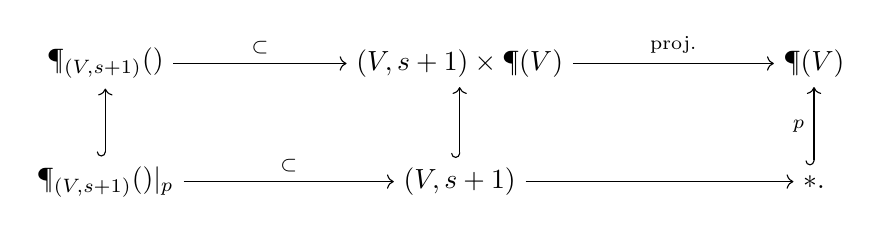
\begin{tikzpicture}[auto]
    \node (A) at (0,1.5) {\(\P_{\G(V,s+1)}(\mcU)\)};
    \node (A') at (0,0) {\(\P_{\G(V,s+1)}(\mcU)|_p\)};
    \node (B) at (4.5,1.5) {\(\G(V,s+1)\times \P(V)\)};
    \node (B') at (4.5,0) {\(\G(V,s+1)\)};
    \node (C) at (9,1.5) {\(\P(V)\)};
    \node (C') at (9,0) {\(*.\)};
    \draw[right hook->] (A') -- (A);
    \draw[right hook->] (B') -- (B);
    \draw[right hook->] (C') -- node {\(\scriptstyle p\)}(C);
    \draw[->] (A) -- node  {\(\scriptstyle \subset\)} (B);
    \draw[->] (B) -- node  {\(\scriptstyle \textrm{proj.}\)} (C);
    \draw[->] (A') -- node  {\(\scriptstyle \subset\)} (B');
    \draw[->] (B') -- (C');
  \end{tikzpicture}
  \]
  \HereEndTikz
  点\(p\)を与える全射も同じ記号\(p:V\to k\)で表す。
  \(\P(V)\)内の次元\(s\)の平面は
  次元\(s+1\)の線形空間\(W\)への全射\(V\to W\)と対応し、
  その平面が点\(p\)を通ることは、
  全射\(V\to W\)の核が\(\ker(p)\)に含まれることを意味する。
  従って、点\(p\)を通る次元\(s\)の平面は、
  次元\(s\)の線形空間\(W'\)への全射
  \(\ker(p)\to W'\)と対応する:
  \[
  \begin{CD}
    0 @>>> \ker(p) @>>> V @>p>> k @>>> 0 \\
    @. @VVV @VVV @| @. \\
    0 @>>> W' @>>> W @>>> k @>>> 0
  \end{CD}
  \]
  \(p:V\to k\)は\(\P(V)\)上のトートロジカルな全射
  \(V_{\P(V)}\to \OO{\P(V)}(1)\)の点\(p\)へのpull-backであり、
  従って\(\ker(p)\)は\(\Omega_{\P(V)}(1)\)の点\(p\)へのpull-backであることに注意する
  (cf. \cite[Remark 4]{YJ})。
  以上より、\(\P(V)\)上の多様体の同型
  \[
  \P_{\G(V,s+1)}(\mcU) \cong \G_{\P(V)}(\Omega_{\P(V)}(1),s)
  \]
  が得られる。

  \autoref{lem: Grass}の証明を完了するため、
  \(\P_{\G(V,s+1)}(\mcU)\subset \G(V,s+1)\times \P(V)\)と
  \(\G(V,s+1)\times X\)の交差を考える。
  \(Y \dfn \P_{\G(V,s+1)}(\mcU) \cap (\G(V,s+1)\times X)\)と置く
  (スキーム論的交差)。
  射影\(Y\to X\)はグラスマン束\(\G_{\P(V)}(\Omega_{\P(V)}(1),s)\to \P(V)\)の
  \(X\)への引き戻しであるから、
  \(Y\cong \G_X(\Omega_{\P(V)}(1)|_X,s)\)である。
  従って
  \[\dim Y = d + s(r-s) = rs-s^2+d\]
  となることがわかる。
  射影\(f:Y\to \G(V,s+1)\)の像\(\im(f)\)は、
  ちょうど\(X\)と交わる\(s\)次元の平面\(H \subset \P(V)\)
  を閉点とする\(\G(V,s+1)\)の閉部分多様体であり、
  さらに各点\([H]\in \im (f)\)での\(f\)のfiberは
  \(H\cap X\)と同型である。
  \[
  \begin{CD}
    Y @>>> \G(V,s+1) \\
    @AAA @AAA \\
    H\cap X @>>> [H].
  \end{CD}
  \]

  \(\dim (\G(V,s+1)) = (r-s)(s+1) = rs-s^2+r-s\)であることに注意する。
  \ref{enumi: lem: Grass empty}を示す。
  \(d< r-s\)なので、
  \(\dim Y < \dim(\G(V,s+1))\)であり、
  特に、射影\(f:Y\to \G(V,s+1)\)の像は真の閉部分集合である。
  このことは\ref{enumi: lem: Grass empty}を示している。
  \ref{enumi: lem: Grass finite}を示す。
  \(d+s=r\)なので\(X\)と次元\(s\)の任意の平面\(\subset \P(V)\)が交わることから、
  射影\(f:Y\to \G(V,s+1)\)は全射である。
  一方、\(\dim Y = rs-s^2+d = rs-s^2+r-s = \dim(\G(V,s+1))\)であるから、
  \(f\)は生成点で有限である。
  すなわち、\(\G(V,s+1)\)のある開集合上で\(f\)のfiberは有限集合となる。
  このことは\ref{enumi: lem: Grass finite}を示している。
  以上で\autoref{lem: Grass}の証明を完了する。
\end{proof}


\autoref{lem: Grass} \ref{enumi: lem: Grass empty}をより詳しく調べる。

\begin{lem}\label{lem: Grass 1pt}
  \(V\)を次元\(r+1\)の線形空間、
  \(0 < s < r\)を整数、
  \(X\subset \P(V)\)を次元\(d < r-s\)の閉部分多様体とする。
  このとき、\(X\)と交わる\(\P(V)\)内の次元\(s\)の平面のうち
  ほとんどは\(X\)と一点で交わる。
\end{lem}


\begin{proof}
  \(2\)点以上で交わる次元\(s\)の平面の集合を調べる。
  \(\Hilb^2(X)\)を\(X\)上の\(2\)点のHilbertスキーム、
  \(\mcU\subset \Hilb^2(X)\times X\)を普遍的な閉部分スキーム、
  つまり長さ\(2\)の閉部分スキーム\(Z\subset X\)に対応する点\([Z]\in \Hilb^2(X)\)上で
  \HereBeginTikz
  \[
  \begin{tikzpicture}[auto]
    \node (A) at (0,1.5) {\(\mcU\)};
    \node (A') at (0,0) {\(\mcU|_{[Z]}\cong Z\)};
    \node (B) at (4.5,1.5) {\(\Hilb^2(X)\times X\)};
    \node (B') at (4.5,0) {\(X\)};
    \node (C) at (9,1.5) {\(\Hilb^2(X)\)};
    \node (C') at (9,0) {\(*\)};
    \draw[right hook->] (A') -- (A);
    \draw[right hook->] (B') -- (B);
    \draw[right hook->] (C') -- node {\(\scriptstyle [Z]\)}(C);
    \draw[->] (A) -- node  {\(\scriptstyle \subset\)} (B);
    \draw[->] (B) -- node  {\(\scriptstyle p\)} (C);
    \draw[->] (A') -- node  {\(\scriptstyle \subset\)} (B');
    \draw[->] (B') -- (C');
  \end{tikzpicture}
  \]
  \HereEndTikz
  となる閉部分スキームとする。
  ただし\(p:\Hilb^2(X)\times X\to \Hilb^2(X)\)は射影である。
  特に合成\(\mcU\subset \Hilb^2(X)\times X\xrightarrow{p} \Hilb^2(X)\)は
  有限平坦射でランク\(2\)である。
  閉埋め込み\(X\subset \P(V)\)を与える全射\(V_X\to L\)を
  \(\Hilb^2(X)\times X\)上へpull-backすれば、
  射の列
  \[
  V_{\Hilb^2(X)\times X} \to L_{\Hilb^2(X)\times X} \to L_\mcU
  \]
  を得る。
  これを射影\(p\)で\(\Hilb^2(X)\)上へpushすれば、
  ランク\(2\)の局所自由層への射
  \[
  \Psi: V_{\Hilb^2(X)}\to p_*(L_\mcU)
  \]
  を得る。
  \(V_X\to L\)が閉埋め込みを与えることから
  (各\(\Hilb^2(X)\)の閉点の上に基底変換して確かめることで)
  射\(\Psi\)が全射であることがわかる。


  各長さ\(2\)の閉部分スキーム\(Z\subset X\)に対し、
  全射\(\Psi_Z:V\to L_Z\)が\(\P(V)\)内の直線を定める。
  全射\(V\to W\)がこの直線を含む次元\(s\)の平面\(\subset \P(V)\)を定めるとする。
  このとき次元\(s-1\)の線形空間への全射
  \(\ker(\Psi_Z)\to W'\)が引き起こされる:
  \[
  \begin{CD}
    0 @>>> \ker(\Psi_Z) @>>> V @>\Psi_Z >> L_Z @>>> 0 \\
    @. @VVV @VVV @| @. \\
    0 @>>> W' @>>> W @>>> L_Z @>>> 0.
  \end{CD}
  \]
  逆に次元\(s-1\)の線形空間への全射\(\ker(\Psi_Z)\to W'\)は
  包含射\(\ker(\Psi_Z)\subset V\)でpush-outをとることで
  次元\(s+1\)の線形空間への全射\(V\to W\)を引き起こし、
  これらは1:1に対応する。
  \(\Hilb^2(X)\)上の包含射
  \(\ker(\Psi)\subset V_{\Hilb^2(X)}\)はグラスマン束の間の閉埋め込み
  \[
  \G_{\Hilb^2(X)}(\ker(\Psi),s-1)\subset \G(V,s+1)\times \Hilb^2(X)
  \]
  を引き起こすが、
  以上の議論により、各閉点\([Z]\in \Hilb^2(X)\)のfiberは
  \HereBeginTikz
  \[
  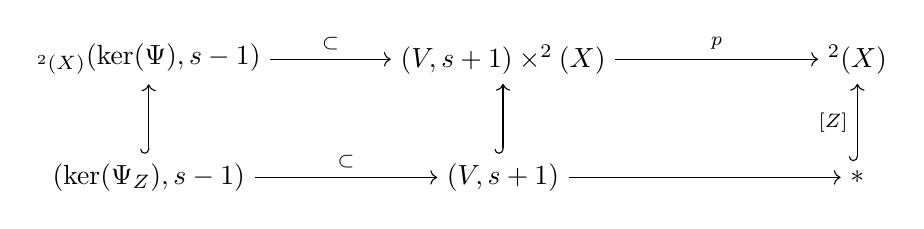
\begin{tikzpicture}[auto]
    \node (A) at (0,1.5) {\(\G_{\Hilb^2(X)}(\ker(\Psi),s-1)\)};
    \node (A') at (0,0) {\(\G(\ker(\Psi_Z),s-1)\)};
    \node (B) at (4.5,1.5) {\(\G(V,s+1)\times \Hilb^2(X)\)};
    \node (B') at (4.5,0) {\(\G(V,s+1)\)};
    \node (C) at (9,1.5) {\(\Hilb^2(X)\)};
    \node (C') at (9,0) {\(*\)};
    \draw[right hook->] (A') -- (A);
    \draw[right hook->] (B') -- (B);
    \draw[right hook->] (C') -- node {\(\scriptstyle [Z]\)}(C);
    \draw[->] (A) -- node  {\(\scriptstyle \subset\)} (B);
    \draw[->] (B) -- node  {\(\scriptstyle p\)} (C);
    \draw[->] (A') -- node  {\(\scriptstyle \subset\)} (B');
    \draw[->] (B') -- (C');
  \end{tikzpicture}
  \]
  \HereEndTikz
  となり、すなわち、
  \(\P(V)\)内の次元\(s\)の平面のうち
  \(Z\)の定める\(\P(V)\)内の直線を通るものたちをパラメタライズする多様体が現れる。
  従って、射影\(g:\G_{\Hilb^2(X)}(\ker(\Psi),s-1)\to \G(V,s+1)\)の像は
  ちょうど\(X\)と二点以上で交わる次元\(s\)の平面たちからなる多様体である。
  特に、射影\(f:\G_X(\Omega_{\P(V)}(1)|_X,s)\to \G(V,s+1)\)の像に含まれる
  (\(f\)については\autoref{lem: Grass}の証明中を参照)。

  \(X\subset \P(V)\)を超平面で\(d\)回切ったのちできる\(0\)次元スキームの
  ある点を選び、その点を通るように異なる超平面をいくつか選ぶことで、
  \(f\)のあるfiberが\(0\)次元であることがわかる。
  従ってfiberの次元の上半連続性 (cf. \cite[Exercise II.3.22]{Ha}) より
  \(f\)はgenerically finiteであることがわかる。
  従って\(\dim (\im (f)) = \dim (\G_X(\Omega_{\P(V)}(1)|_X,s))\)である。
  また、
  \begin{align*}
    \dim (\G_{\Hilb^2(X)}(\ker(\Psi),s-1))
    &= 2d + (s-1)((r+1-2)-(s-1)) = 2d + (s-1)(r-s) \\
    &< d + s(r-s) = \dim (\G_X(\Omega_{\P(V)}(1)|_X,s)) = \dim (\im (f))
  \end{align*}
  であるから、
  \(\im(g)\)は\(\im(f)\)の真の閉部分集合となる。
  このことは
  \(X\)と交わる次元\(s\)の平面のうち
  ほとんどは\(X\)と\(1\)点で交わるということを示している。
  以上で\autoref{lem: Grass 1pt}の証明を完了する。
\end{proof}




\section{証明}



この節では、冒頭の問題\cite[演習 I.4.9]{Ha}を少し一般的な形で証明する。

\begin{prop}
  \(X\subset \P^N\)を\(r\)次元の部分多様体、
  \(s\)を\(N\geq r+s+2\)となる自然数とする。
  次を満たす線形部分多様体\(\P^s\subset \P^N\)を閉点に持つ
  \(\G(N+1,s+1)\)の部分空間はある稠密開集合を含む:
  \begin{itemize}
    \item
    \(\P^s\subset \P^N\)は\(X\subset \P^N\)と交わらず、
    \(\P^s\)に沿った射影\(\P^N\dto \P^{N-s}\)は
    \(X\)から像\(X'\subset \P^{N-s}\)への双有理射を引き起こす。
  \end{itemize}
\end{prop}


\begin{proof}
  \(V=H^0(\P^N,\OO{\P^N}(1))\)と置き、\(\P^N=\P(V)\)と書く。
  \(\G(V,s+1)\)上のトートロジカルな全射を
  \(V_{\G(V,s+1)}\to \mcU\)と置き、その核を\(\mcK\)とする。
  閉埋め込み\(\P_{\G(V,s+1)}(\mcU)\subset \G(V,s+1)\times \P(V)\)
  に沿った爆発を\(B\)と置くと、
  \cite[Corollary 9]{YJ}より\(B\)は
  \(R\dfn \P_{\G(V,s+1)}(\mcK)\)上の\(\P^{s+1}\)-束であり、
  \(R\)上の\(\P^{s+1}\)-束の構造は、
  \[
  \begin{CD}
    0 @>>> \mcK_R @>>> V_R @>>> \mcU_R @>>> 0 \\
    @. @VVV @VVV @| @. \\
    0 @>>> \OO{R/\G(V,s+1)}(1) @>>> \mcE @>>> \mcU_R @>>> 0
  \end{CD}
  \]
  という完全列の間の射ができるようなランク\(s+2\)の\(R\)上の局所自由層\(\mcE\)により
  \(B\cong \P_R(\mcE)\)で与えられている。
  全射\(V_R\to \mcE\)はグラスマン多様体への射
  \(q:\P_{\G(V,s+1)}(\mcK) \to \G(V,s+2)\)を引き起こすことに注意する。
  \(\G(V,s+1)\times \P(V)\)における\(\P_{\G(V,s+1)}(\mcU)\)と
  \(\G(V,s+1)\times X\)のスキーム論的交差を\(D\)と置き、
  \(\G(V,s+1)\times X\)の\(D\)に沿った爆発を\(B_X\)と置く。
  以下の図式ができる (以下のように射に名前をつける):
  \HereBeginTikz
  \[
  \begin{tikzpicture}[auto]
    \node (A) at (0,1.5) {\(B_X\)};
    \node (A') at (0,0) {\(\G(V,s+1)\times X\)};
    \node (B) at (4.5,1.5) {\(B\)};
    \node (B') at (4.5,0) {\(\G(V,s+1)\times \P(V)\)};
    \node (C) at (9,1.5) {\(R\)};
    \node (C') at (9,0) {\(\G(V,s+1)\)};
    \node (D) at (12,1.5) {\(\G(V,s+2)\)};
    \draw[right hook->] (A) -- (B);
    \draw[right hook->] (A') -- (B');
    \draw[->] (B) -- node {\(\scriptstyle \P^{s+1}\text{-束}\)} (C);
    \draw[->] (B) -- node[swap] {\(\scriptstyle \sigma\)} (C);
    \draw[->] (B') -- node {\(\scriptstyle \text{proj.}\)} (C');
    \draw[->] (A) -- (A');
    \draw[->] (B) -- node {\(\scriptstyle \pi\)} (B');
    \draw[->] (C) -- node {\(\scriptstyle p\)} (C');
    \draw[->] (C) -- node {\(\scriptstyle q\)}(D);
  \end{tikzpicture}
  \]
  \HereEndTikz
  閉点\(x\in \P_{\G(V,s+1)}(\mcK)\)は\(p,q\)での像をとることで
  \(p(x)\in \G(V,s+1)\)に対応する\(\P(V)\)の\(s\)次元平面\(H_{p(x)}\)と
  \(q(x)\in \G(V,s+2)\)に対応する\(\P(V)\)の\(s+1\)次元平面\(H_{q(x)}\)を定め、
  \(H_{p(x)}\subset H_{q(x)}\)となる。
  さらに\(\sigma\)での\(x\)のfiber \(\sigma^{-1}(x)\)の\(\pi\)での像は、
  ちょうど\(H_{q(x)}\)となる、つまり
  \(\pi(\sigma^{-1}(x)) = H_{q(x)}\)である。

  \(Z\subset \G(V,s+2)\)を\(X\)と\textbf{交わる}\(s+1\)次元平面のなす閉部分集合とする。
  各\(s\)次元平面\(H\subset \P(V)\)に対して、
  \(H\)に含まれない\(X\)の点が存在しないならば、\(X\subset H\)であるから、
  点\([H]\in \G(V,s+1)\)のfiber \(p^{-1}([H])\)と\(q^{-1}(Z)\)は明らかに交わり、
  \(H\)に含まれない\(X\)の点が存在するならば、
  その点をとることで構成される新たな\(s+1\)次元平面\(H'\)の定める\(R\)の点は
  \(q^{-1}(Z)\)と\(p^{-1}([H])\)のどちらにも含まれる。
  従って射\(p|_{q^{-1}(Z)}:q^{-1}(Z)\to \G(V,s+1)\)は全射である。
  \(N \geq r+s+2\)であるから、\autoref{lem: Grass 1pt}より、
  \(X\)とちょうど\(1\)点で交わる\(s+1\)次元平面からなる稠密開集合\(V\subset Z\)がある。
  \(V\subset Z\)は稠密であり、
  \(p|_{q^{-1}(Z)}:q^{-1}(Z)\to \G(V,s+1)\)は全射であるから、
  \(p(q^{-1}(V))\subset \G(V,s+1)\)は稠密な構成可能集合であり、特に開である。

  \(N \geq r+s+2\)であるから、\autoref{lem: Grass}より、
  \(X\)と交わらない\(s\)次元平面のなす
  空でない開集合\(U\subset \G(V,s+1)\)がある。
  各点\([H]\in U\)に対し、
  \(H\)を軸とする射影\(\P(V)\dto \P(\mcK_{[H]})\cong \P^{N-s}\)
  を\(X\)に制限したものは
  (\(H\)が\(X\)と交わらないことから)
  \(\G(V,s+1)\)上の二つの射\(B_X\to B\to R\)の
  合成射\(r:B_X\to R\)の
  点\([H]\)でのfiberに他ならない。
  点\(x\in R\)について
  \begin{itemize}
    \item[ \ ] \(x\in \im (r:B_X\to R)\)
    \item[\(\iff\)] \(\pi(\sigma^{-1})\cap X \neq \emptyset\)
    \item[\(\iff\)] \(X\)と\(q(x)\)に対応する\(\P(V)\)の\(s+1\)次元平面が交わる
    \item[\(\iff\)] \(x\in q^{-1}(Z)\)
  \end{itemize}
  であるから、\(\im (r) = q^{-1}(Z)\)となる。
  点\(x\in q^{-1}(V)\)の\(r:B_X\to R\)でのfiberは
  ちょうど\(X\)と\(q(x)\)に対応する\(\P(V)\)の\(s+1\)次元平面のスキーム論的交差であり、
  すなわちスキーム論的に\(1\)点である。
  従って、\(r\)は空でない開集合\(r^{-1}(q^{-1}(V))\subset B_X\)上で同型射である。

  \(W\dfn p(q^{-1}(V))\cap U\subset \G(V,s+1)\)と置く。
  各点\([H]\in W\)に対して、
  \(p^{-1}([H])\cap q^{-1}(V)\neq \emptyset\)であるから
  \(H\)を軸とする射影\(r_H:X\to \P(\mcK_{[H]})\cong \P^{N-s}\)は像への双有理射である。
  また、\(W\subset U\)であるから、\(s\)次元平面\(H\)は\(X\)とは交わらない。
  よって\(W\)は所望の開集合である。
  以上で証明を完了する。
\end{proof}








\begin{thebibliography}{9}
  \bibitem[Ha]{Ha}
  R.Hartshorne,
  \textit{Algebraic Geometry}.
  Springer-Verlag, New Tork, 1977. Graduate Text in Mathematics, No. 52.
  \bibitem[ゆ]{YJ}
  ゆじノート,
  \textit{Blowing Up along Linear Subvariety}.
\end{thebibliography}


\end{document}
